\chapter{Теоретичні відомості}
\section{Постановка задачі}
У цьому розділі буде розглянуто необхідний математичний апарат та теоретичні відомості стосовно проблеми яка лежить в основі даної магістерської дисертації. Розглянемо основне твердження теореми Шпернера та усі супутні визначення та твердження необхідні для вирішення поставленної задачі.

\textbf{Теорема Шпернера}
\par Нехай $ M = \{1,...,n\} $ множина яка скаладється з елементів натурального ряду,
$M_1,...,M_k$ - підмножини множини $ M $ такі, що $ \forall M_i,M_j: M_i \not\subset M_j $, 
тоді виконується дуже проста нерівність $k \leq {C_n}^{[n/2]}$, де $ k $ - це кількість множин у наборі $M_1,...,M_k$, $ n $ - загальна кількість елементів множини $ M $ (тобто потужність множини $ M $, далі будемо позначати як $ |M| $), $ {C_n}^{[n/2]} $ - біноміальний коефіцієнт, $ [n/2] $ - ціла частина від діллення $ n $ навпіл.
\newpage
\\
Це питання відповідь на яке ми знайдемо після того як трохи попишемо текст. Тут текст, як же він буде відображатись? Це питання відповідь на яке ми знайдемо після того як трохи попишемо текст.Тут текст, як же він буде відображатись?
\\
\begin{center}
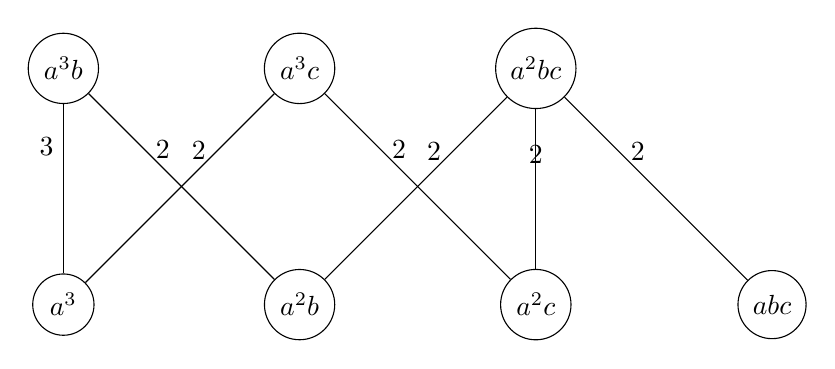
\begin{tikzpicture}[node distance={30mm}, main/.style = {draw, circle}] 
\node[main] (1) {$a^3b$}; 
\node[main] (2) [right of=1] {$a^3c$}; 
\node[main] (3) [right of=2] {$a^2bc$}; 
\node[main] (4) [below of=1] {$a^3$}; 
\node[main] (5) [below of=2] {$a^2b$}; 
\node[main] (6) [below of=3] {$a^2c$}; 
\node[main] (7) [right of=6] {$abc$}; 

\draw (1) -- node[pos=0.25, left] {3} (4); 
\draw (1) -- node[pos=0.4, above] {2} (5); 
\draw (2) -- node[pos=0.4, above] {2}(4); 
\draw (2) -- node[pos=0.4, above] {2}(6); 
\draw (3) -- node[pos=0.4, above] {2}(5); 
\draw (3) -- node[pos=0.4, above] {2}(6); 
\draw (3) -- node[pos=0.4, above] {2}(7); 
\end{tikzpicture} 
\end{center}
\newpage
\\
Це питання відповідь на яке ми знайдемо після того як трохи попишемо текст.Тут текст, як же він буде відображатись? Це питання відповідь на яке ми знайдемо після того як трохи попишемо текст.Тут текст, як же він буде відображатись? Це питання відповідь на яке ми знайдемо після того як трохи попишемо текст. Тут текст, як же він буде відображатись? Це питання відповідь на яке ми знайдемо після того як трохи попишемо текст. Тут текст, як же він буде відображатись? Це питання відповідь на яке ми знайдемо після того як трохи попишемо текст. Тут текст, як же він буде відображатись? Це питання відповідь на яке ми знайдемо після того як трохи попишемо текст. Це питання відповідь на яке ми знайдемо після того як трохи попишемо текст. Це питання відповідь на яке ми знайдемо після того як трохи попишемо текст.
\\
	Hile Hitler!
\subsection{Попередні роботи} 
\subsection{Визначення}
\section{Розв'язок}
